%% abtex2-modelo-trabalho-academico.tex, v-1.9.2 laurocesar
%% Copyright 2012-2014 by abnTeX2 group at http://abntex2.googlecode.com/ 
%%
%% This work may be distributed and/or modified under the
%% conditions of the LaTeX Project Public License, either version 1.3
%% of this license or (at your option) any later version.
%% The latest version of this license is in
%%   http://www.latex-project.org/lppl.txt
%% and version 1.3 or later is part of all distributions of LaTeX
%% version 2005/12/01 or later.
%%
%% This work has the LPPL maintenance status `maintained'.
%% 
%% The Current Maintainer of this work is the abnTeX2 team, led
%% by Lauro César Araujo. Further information are available on 
%% http://abntex2.googlecode.com/
%%
%% This work consists of the files abntex2-modelo-trabalho-academico.tex,
%% abntex2-modelo-include-comandos and abntex2-modelo-references.bib
%%

% ------------------------------------------------------------------------
% ------------------------------------------------------------------------
% abnTeX2: Modelo de Trabalho Academico (tese de doutorado, dissertacao de
% mestrado e trabalhos monograficos em geral) em conformidade com 
% ABNT NBR 14724:2011: Informacao e documentacao - Trabalhos academicos -
% Apresentacao
% ------------------------------------------------------------------------
% ------------------------------------------------------------------------

\documentclass[
	% -- opções da classe memoir --
	12pt,				% tamanho da fonte
	openright,			% capítulos começam em pág ímpar (insere página vazia caso preciso)
	twoside,			% para impressão em verso e anverso. Oposto a oneside
	a4paper,			% tamanho do papel. 
	% -- opções da classe abntex2 --
	%chapter=TITLE,		% títulos de capítulos convertidos em letras maiúsculas
	%section=TITLE,		% títulos de seções convertidos em letras maiúsculas
	%subsection=TITLE,	% títulos de subseções convertidos em letras maiúsculas
	%subsubsection=TITLE,% títulos de subsubseções convertidos em letras maiúsculas
	% -- opções do pacote babel --
	english,			% idioma adicional para hifenização
	french,				% idioma adicional para hifenização
	spanish,			% idioma adicional para hifenização
	brazil				% o último idioma é o principal do documento
	]{abntex2}

% ---
% Pacotes básicos 
% ---
\usepackage{lmodern}			% Usa a fonte Latin Modern			
\usepackage[T1]{fontenc}		% Selecao de codigos de fonte.
\usepackage[utf8]{inputenc}		% Codificacao do documento (conversão automática dos acentos)
\usepackage{lastpage}			% Usado pela Ficha catalográfica
\usepackage{indentfirst}		% Indenta o primeiro parágrafo de cada seção.
\usepackage{color}				% Controle das cores
\usepackage{graphicx}			% Inclusão de gráficos
\usepackage{microtype} 			% para melhorias de justificação
\usepackage{amsmath}
\usepackage{graphicx}
\usepackage{wrapfig}
\usepackage{lscape}
\usepackage{rotating}
\usepackage{epstopdf}
\usepackage[section]{placeins}
% ---
		
% ---
% Pacotes adicionais, usados apenas no âmbito do Modelo Canônico do abnteX2
% ---
\usepackage{lipsum}				% para geração de dummy text
% ---

% ---
% Pacotes de citações
% ---
\usepackage[brazilian,hyperpageref]{backref}	 % Paginas com as citações na bibl
\usepackage[alf]{abntex2cite}	% Citações padrão ABNT
\usepackage{relsize}
% --- 
% CONFIGURAÇÕES DE PACOTES
% --- 

% ---
% Configurações do pacote backref
% Usado sem a opção hyperpageref de backref
\renewcommand{\backrefpagesname}{Citado na(s) página(s):~}
% Texto padrão antes do número das páginas
\renewcommand{\backref}{}
% Define os textos da citação
\renewcommand*{\backrefalt}[4]{
	\ifcase #1 %
		Nenhuma citação no texto.%
	\or
		Citado na página #2.%
	\else
		Citado #1 vezes nas páginas #2.%
	\fi}%
% ---

% ---
% Informações de dados para CAPA e FOLHA DE ROSTO
% ---
\titulo{Information Measures Applied to the Analysis of Complex Networks in Epilepsy}
\autor{Viviane Silveira Gonçalves Martins Tenório}
\local{Campina Grande, Brazil}
\data{2018}
\orientador{Francisco Marcos de Assis}
%\coorientador{Equipe \abnTeX}
\instituicao{%
  Federal University of Campina Grande
  \par
  Electrical Engineering Department
  \par
  Bachelor Program in Electrical Engineering}
\tipotrabalho{Thesis}
% O preambulo deve conter o tipo do trabalho, o objetivo, 
% o nome da instituição e a área de concentração 
\preambulo{Trabalho de Conclusão de Curso submetido à Unidade Acadêmica de Engenharia Elétrica da Universidade Federal de Campina Grande como parte dos requisitos necessários para a obtenção do grau de Bacharel em Ciências no Domínio da Engenharia Elétrica.}
% ---


% ---
% Configurações de aparência do PDF final

% alterando o aspecto da cor azul
\definecolor{blue}{RGB}{41,5,195}

% informações do PDF
\makeatletter
\hypersetup{
     	%pagebackref=true,
		pdftitle={\@title}, 
		pdfauthor={\@author},
    	pdfsubject={\imprimirpreambulo},
	    pdfcreator={LaTeX with abnTeX2},
		pdfkeywords={abnt}{latex}{abntex}{abntex2}{trabalho acadêmico}, 
		colorlinks=true,       		% false: boxed links; true: colored links
    	linkcolor=blue,          	% color of internal links
    	citecolor=blue,        		% color of links to bibliography
    	filecolor=magenta,      		% color of file links
		urlcolor=blue,
		bookmarksdepth=4
}
\makeatother
% --- 

% --- 
% Espaçamentos entre linhas e parágrafos 
% --- 

% O tamanho do parágrafo é dado por:
\setlength{\parindent}{1.3cm}

% Controle do espaçamento entre um parágrafo e outro:
\setlength{\parskip}{0.2cm}  % tente também \onelineskip

% ---
% compila o indice
% ---
\makeindex
% ---

% ----
% Início do documento
% ----
\begin{document}

% Retira espaço extra obsoleto entre as frases.
\frenchspacing 

% ----------------------------------------------------------
% ELEMENTOS PRÉ-TEXTUAIS
% ----------------------------------------------------------
% \pretextual

% ---
% Capa
% ---
\imprimircapa
% ---

% ---
% Folha de rosto
% (o * indica que haverá a ficha bibliográfica)
% ---
\imprimirfolhaderosto*
% ---

% ---
% Inserir a ficha bibliografica
% ---

% Isto é um exemplo de Ficha Catalográfica, ou ``Dados internacionais de
% catalogação-na-publicação''. Você pode utilizar este modelo como referência. 
% Porém, provavelmente a biblioteca da sua universidade lhe fornecerá um PDF
% com a ficha catalográfica definitiva após a defesa do trabalho. Quando estiver
% com o documento, salve-o como PDF no diretório do seu projeto e substitua todo
% o conteúdo de implementação deste arquivo pelo comando abaixo:
%
% \begin{fichacatalografica}
%     \includepdf{fig_ficha_catalografica.pdf}
% \end{fichacatalografica}
%\begin{fichacatalografica}
%	\vspace*{\fill}					% Posição vertical
%	\hrule							% Linha horizontal
%	\begin{center}					% Minipage Centralizado
%	\begin{minipage}[c]{12.5cm}		% Largura
%	
%	\imprimirautor
%	
%	\hspace{0.5cm} \imprimirtitulo  / \imprimirautor. --
%	\imprimirlocal, \imprimirdata-
	
%	\hspace{0.5cm} \pageref{LastPage} p. : il. (algumas color.) ; 30 cm.\\
%	
%	\hspace{0.5cm} \imprimirorientadorRotulo~\imprimirorientador\\
%	
%	\hspace{0.5cm}
%	\parbox[t]{\textwidth}{\imprimirtipotrabalho~--~\imprimirinstituicao,
%	\imprimirdata.}\\
%	
%	\hspace{0.5cm}
%		1. Palavra-chave1.
%		2. Palavra-chave2.
%		I. Orientador.
%		II. Universidade xxx.
%		III. Faculdade de xxx.
%		IV. Título\\ 			
%	
%	\hspace{8.75cm} CDU 02:141:005.7\\
%	
%	\end{minipage}
%	\end{center}
%	\hrule
%\end{fichacatalografica}
% ---

% ---
% Inserir errata
% ---
%\begin{errata}
%Elemento opcional da \citeonline[4.2.1.2]{NBR14724:2011}. Exemplo:

%\vspace{\onelineskip}


% ---

% ---
% Inserir folha de aprovação
% ---

% Isto é um exemplo de Folha de aprovação, elemento obrigatório da NBR
% 14724/2011 (seção 4.2.1.3). Você pode utilizar este modelo até a aprovação
% do trabalho. Após isso, substitua todo o conteúdo deste arquivo por uma
% imagem da página assinada pela banca com o comando abaixo:
%
% \includepdf{folhadeaprovacao_final.pdf}
%
\begin{folhadeaprovacao}

  \begin{center}
    {\ABNTEXchapterfont\large\imprimirautor}

    \vspace*{\fill}\vspace*{\fill}
    \begin{center}
      \ABNTEXchapterfont\bfseries\Large\imprimirtitulo
    \end{center}
    \vspace*{\fill}
    
    \hspace{.45\textwidth}
    \begin{minipage}{.5\textwidth}
        \imprimirpreambulo
    \end{minipage}%
    \vspace*{\fill}
   \end{center}
        
   Trabalho aprovado. \imprimirlocal, 17 de Dezembro de 2018:

   \assinatura{\textbf{\imprimirorientador} \\ Orientador} 
   \assinatura{\textbf{Professora Dra. Luciana Veloso} \\ Convidada}
   %\assinatura{\textbf{Professor} \\ Convidado 2}
   %\assinatura{\textbf{Professor} \\ Convidado 3}
   %\assinatura{\textbf{Professor} \\ Convidado 4}
      
   \begin{center}
    \vspace*{0.5cm}
    {\large\imprimirlocal}
    \par
    {\large\imprimirdata}
    \vspace*{1cm}
  \end{center}
  
\end{folhadeaprovacao}
% ---

% ---
% Dedicatória
% ---
\begin{dedicatoria}
   \vspace*{\fill}
   \centering
   \noindent
   \textit{ Ao meu "V\^o Zez\'e"} \vspace*{\fill}
\end{dedicatoria}
% ---

% ---
% Agradecimentos
% ---
\begin{agradecimentos}
Aos meus pais, Raissa e Fábio, por terem dividido comigo cada pedaço dessa jornada. Pelos conselhos, paciência, força, dedicação. Por terem enxugado minhas lágrimas e meu suor. Pelo sorriso e colo. Por terem me dado muito mais do que eu precisava para chegar até aqui, mas, acima de tudo, por serem meu exemplo. As minhas irmãs, Amanda e Beatriz, por terem "feito elétrica junto comigo" mesmo sem saber fazer uma integral. Pelos filmes, pelas risadas, pelo carinho e apoio incondicional, e principalmente pela fé - que nunca deixaram faltar em mim. Ao meu esposo, Marcus, por ter sido meu maior incentivador. Pela compreensão nos incontáveis "finais de período", por ter sido paz e porto seguro por todos esse anos e por ter sonhado junto comigo cada passo do caminho.

A Bruna, Magda, Melissa e Raissa (em ordem alfabética), por terem sido as melhores companheiras de jornada. Por terem tirado todas as minhas dúvidas, aguentando meus choros, ensinado, compartilhado materiais, experiências e dias de luta. Obrigada por terem feito de elétrica uma experiência que eu vou guardar com carinho.

Agradeço aos meus professores, e em especial a Raimundo Freire por ter aberto um novo mundo de possibilidades para mim. Por ter sido sempre exigente, me ensinado com rigor e com paciência e dedicação. Agradeço ao Prof. Tejo por ter aberto portas para a relização do sonho de pesquisar em engenheira biomédica, pelas conversas e orientações, pelos livros e pela confiança. Ao Prof. Francisco Marcos por ter me orientado na etapa final, sempre retirando de mim o melhor que eu tinha para oferecer, pela conversa amiga e por todos os ensinamentos. Às Profa. Priscilla Castro e Profa. Cristina Ruan, por todo o incentivo e apoio na minha formação extra-curricular e pelo colhimento no departamento de Enfermagem na UFCG, onde pude ganhar mais confiança nos aspectos biológicos deste trabalho.

Ao Hospital Israelita Albert Einstein, e em especial a Birajara Soares, pelo estágio que inspirou e embasou esse trabalho.

Agradeço à CAPES e ao Governo Federal pela possibilidade de ter realizado intercâmbio na Politécnica de Milão, sem o qual esse trabalho não exisitiria.

Agradeço por fim, mas não menos importante, a Deus pela resiliência e inspiração de sempre seguir em frente e não desistir dos meus ideais.


\end{agradecimentos}
% ---

% ---
% Epígrafe
% ---
\begin{epigrafe}
    \vspace*{\fill}
	\begin{flushright}
		\textit{``Um dos indiretos modos de entender é achar bonito. \\
Do lugar onde estou de pé, a vida é muito bonita. \\
Entender é um modo de olhar. 
\\ Porque entender, aliás, é uma atitude. 
\\ O que a gente não entende, se resolve com amor.\\
(Clarice Lispector, 1961)}
	\end{flushright}
\end{epigrafe}
% ---

% ---
% RESUMOS
% ---

% resumo em português
\setlength{\absparsep}{18pt} % ajusta o espaçamento dos parágrafos do resumo
\begin{resumo}
 
 A análise de sinais biológicos requer forte fundamentação matemática e estatística. No escopo de neuropatologias, a teoria da informação é uma ferramenta bastante utilizada para análise dos sinais eletroengefalográficos. O presente trabalho propõe-se a identificar os hubs presentes durante o período ictal de episódios de epilepsia a partir de duas medidas de informação: o "Phase Locking Value" (ou PLV) e a Entropia de Transferência. Percebeu-se que, dada a sua natureza direcional, a entropia de transferência apresentou resultados mais específicos para a identificação da região anatômica dos "hubs".
 
 

 \textbf{Palavras-chaves}: Sinais Biológicos, EEG, Phase Locking Value, Entropia de Transferência.
\end{resumo}

% resumo em inglês
\begin{resumo}[Abstract]
 \begin{otherlanguage*}{english}
  The analysis of biological signals has a strong mathematical and statistical foundation. In the scope of neuropathologies, information theory is a widely used tool for the analysis of electroencephalograhy signals. The present work proposes to identify the hubs present during the ictal period of epilepsy episodes from two information measures: Phase Locking Value (PLV) and Transfer Entropy. It was noticed that, given its directional nature, the transfer entropy presented more specific results for the identification of the anatomical region of the hubs.

   \vspace{\onelineskip}
 
   \noindent 
   \textbf{Key-words}: Biological Signals, EEG, Phase Locking Value, Transfer Entropy.
 \end{otherlanguage*}
\end{resumo}


% ---
% inserir lista de ilustrações
% ---
\pdfbookmark[0]{\listfigurename}{lof}
\listoffigures*
\cleardoublepage
% ---

% ---
% inserir lista de tabelas
% ---
\pdfbookmark[0]{\listtablename}{lot}
\listoftables*
\cleardoublepage
% ---

% ---
% inserir lista de abreviaturas e siglas
% ---
\begin{siglas}
  \item[BC] Betweeness Centrality
  \item[EEG] Eletroencefalograma
  \item[PLV] Phase Locking Value
  \item[TE] Transfer Entropy
\end{siglas}
% ---

% ---
% inserir lista de símbolos
% ---
%\begin{simbolos}
%  \item[$ \Gamma $] Letra grega Gama
%  \item[$ \Lambda $] Lambda
%  \item[$ \zeta $] Letra grega minúscula zeta
%  \item[$ \in $] Pertence
%\end{simbolos}
% ---

% ---
% inserir o sumario
% ---
\pdfbookmark[0]{\contentsname}{toc}
\tableofcontents*
\cleardoublepage
% ---



% ----------------------------------------------------------
% ELEMENTOS TEXTUAIS
% ----------------------------------------------------------
\textual

% ----------------------------------------------------------
% Introdução (exemplo de capítulo sem numeração, mas presente no Sumário)
% ----------------------------------------------------------
\chapter*[Introdução]{Introdução}
\addcontentsline{toc}{chapter}{Introdução}
% ----------------------------------------------------------
A epilepsia é um mau funcionamento do cérebro que afeta mais de 50 milhões de
pessoas em todo o mundo. Crises epilépticas são geralmente caracterizadas por um disparo sincronizado anormal de neurônios envolvidos no processo epiléptico. Na epilepsia humana, os mecanismos exatos subjacentes à geração de crises ainda são incertos, assim como os mecanismos subjacentes à disseminação e término das crises \cite{lehnertz2009synchronization}. Há agora evidências crescentes de que uma melhor compreensão do processo epiléptico pode ser alcançada através da análise de redes cerebrais epilépticas e através da análise de interações destas tais redes \cite{boccaletti2001unifying}.

A teoria da informação, estabelecida em 1948 por um artigo de Claude Shannon \cite{shannon1948mathematical}, trouxe conhecidas contribuições às comunicações, à ciência da computação, à probabilidade e à estatística \cite{cover2012elements}. Alguns de seus conceitos, como o de informação mútua, informação direcional e entropia de transferência, podem ser aplicados em diversos sistemas, não apenas aqueles de sinais naturais, tais quais os sistemas biológicos e climáticos, como também os de sinais “artificiais”, tais quais os sistemas econômicos e de processamento industrial \cite{juliana}.

A repetida coincidência de sinais ao longo do tempo, ou seja, o movimento síncrono duradouro, é geralmente consequência da sincronização \cite{kraskov2004synchronization}. No início do século XX, os fenômenos de sincronização foram estudados por W.H. Eccles e J.H. Vincent no contexto da engenharia elétrica. Em seus experimentos o ajuste das frequências de dois triodos acoplados geradores com frequências inicialmente diferentes foi demonstrado \cite{eccles}. Esse foi um dos primeiros experimentos relacionados à teoria de sincronização de fase, teoria que posteriormente embasaria o Phase Locking value (PLV).

Alguns anos mais tarde, E. Appleton \cite{appleton1922automatic} e B. van der Pol estenderam os experimentos de Eccles e Vincent e também realizaram investigações teóricas sobre os fenômenos de sincronização. Van der Pol então concebeu sua famosa equação, o primeiro exemplo de um sistema auto-oscilante não-linear \cite{van1927vii}. Além disso, van der Pol, juntamente com van der Mark, propuseram um modelo elétrico do coração consistindo de três osciladores de relaxamento acoplados \cite{van1928lxxii}. 

Uma nova etapa de estudos de sincronização começou algumas décadas após a descoberta do caos determinístico \cite{lorenz1963mechanics}. No início dos anos 80, a noção de sincronização foi estendida à caso de osciladores caóticos em interação \cite{PhysRevLett.64.821}. 

 Muitas vezes, as informações mais confiáveis sobre sistemas em interação são contidos nas fases dos sinais. Uma diferença de fase fixa e contínua em um intervalo de tempo é fundamental para sincronização de fase \cite{kraskov2004synchronization}. 

A variedade de conceitos de sincronização estimulou o desenvolvimento de   diferentes abordagens visando uma quantificação do grau de sincronização entre dois sistemas, ou melhor, entre duas séries temporais medidas a partir dos respectivos sistemas. 

A informação mútua é uma delas \cite{cover2012elements}. É zero estatísticamente se e somente se duas variáveis aleatórias são estritamente independentes. Duas das técnicas mais importantes para calcular numericamente a informaçao mútua utilizam a transformada de Hilbert \cite{PhysRevLett.Rosenblum} ou a transformada wavelet \cite{Lachaux}.

Uma aplicação  para medidas de sincronização é o estudo da dinâmica neuronal, uma vez que os fenômenos de sincronização têm sido cada vez mais reconhecidos como uma característica fundamental para estabelecer a comunicação entre diferentes regiões do cérebro \cite{varela2001brainweb}. Por outro lado, a sincronização também desempenha um papel importante nos processos patológicos como doença de Parkinson ou epilepsia.

Por vezes, registros multicanais usando técnicas de monitoramento intracraniano são utilizados para obter informações suficientes para uma localização inequívoca de uma estrutura geradora de convulsões (foco epiléptico) no cérebro.

A investigação dessas gravações por meio de técnicas de análise de séries temporais lineares e não-lineares pode ajudar a entender melhor a dinâmica espaço-temporal do cérebro epilético \cite{LEHNERTZ1995108}.

Isso  motivou a realização de uma comparação entre a Entropia de Transferência e o PLV (Phase Locking Value) para determinação dos parâmetros de rede propostos por Sporns \cite{sporns2010networks} para determinação do foco epiléptico.

O presente trabalho está organizado conforme segue: no capítulo 1 será apresentada a fundamentação teórica, bem como os conceitos utilizados para a análise dos dados. O capítulo 2 apresenta informações sobre a aquisição dos dados junto ao Hospital Israelita Albert Einstein. No caítulo 3 estão apresentados os resultados e as principais discussões. Ao final tem-se a conclusão e perspectivas de trabalhos futuros.






% ----------------------------------------------------------
% PARTE
% ----------------------------------------------------------
\chapter{Fundamentação Teórica}

 
Os sinais biológicos, após aquisição, são analisados como series temporais. Diversas técnicas são utilizadas atualmente para a análise de séries temporais, mas em se tratando de conectividade (e sincronização) duas vertentes chamam atenção: A transferência de entropia e o Phase Locking Value (PLV).

Ambas teorias foram desenvolvidas quase simultaneamente embora a pimeira, inpirada no trabalho de Shannon, tenha sido a mais amplamente aplicada.

Por se tratar de uma medida não direcional, o PLV não contém o mesmo nível de informação que a transferência de entropia. Porém, a informação contida na fase dos sinais, é evidenciada e a sincronização torna-se proeminente.

Os dois conceitos serão apresentados a seguir, bem como o conceito de redes complexas adotado nesse trabalho. 

As redes cerebrais são invariavelmente complexas, compartilham uma série de características comuns com redes de outros sistemas biológicos e físicos e, portanto, podem ser caracterizadas usando métodos complexos de rede.

Essas características bem como todos os métodos utilizados serão apresentados a seguir.


% ----------------------------------------------------------
\section{Phase Locking Value}
O conceito de sincronização de fases \cite{PhysRevLett.Rosenblum}
baseia-se no estudo de osciladores caóticos e / ou ruidosos, fracamente acoplados e generaliza o fenômeno de travamento de fase (phase locking). A diferença instantânea de fases de dois osciladores sincronizados permanece constante durante o estado de travamento de fase.

Na sincronização de fase, as amplitudes podem não ser correlacionadas \cite{PhysRevLett.Rosenblum}.

A sincronização completa é um estado em que ambos os sistemas oscilatórios se tornam topologicamente idênticos - fases e amplitudes dos dois osciladores estão fortemente correlacionadas. Os diferentes tipos de sincronização aparecem em dependência da força de acoplamento entre os dois sistemas: os processos oscilatórios não são correlacionados quando não há acoplamento entre eles, a sincronização de fase aparece entre os osciladores fracamente acoplados e a sincronização completa aparece quando a força de acoplamento aumenta acima de algum limiar.

 Considerando a definição rigorosa em que a diferença de fase vale para duas fases instantâneas: uma poertencente à série $i$ dada por $\phi_{i,t}$ e outra pertencente à série $j$ dada por $\phi_{j,t}$ em que os índices $m$ e $n$ representam fases únicas, dado  $m=n=1$, em 
$|\Delta\phi_t|=|m\phi_{i,t}-n\phi_{j,t}|$. 
Para calcular a sincronização de fase, é necessário conhecer a fase instantânea de ambos os sinais envolvidos. Aqui, propusemos uma média de energia ponderada de fase em todas as escalas de wavelets. \cite{Rodrigues2014},
\begin{equation}
\phi_\tau=\frac{1}{\Gamma_\tau}\sum_\ell|W_\tau(\ell)|^2\phi_\tau(\ell)\;,
\end{equation}
onde $\phi_\tau (\ell)=\arctan\Im[W_\tau(\ell)]/\Re[W_\tau(\ell)]$, 
$\Gamma_\tau=\sum_\ell|W_\tau(\ell)|^2$ e
\begin{equation}
W_\tau(\ell)=\int_{-\infty}^{\infty}f(t)\psi_\tau(\ell,t)dt\;,
\end{equation}
 a transformada wavelet de uma determinada função $f(t)$ localizada em $\tau$ com escala $\ell$. A função de kernel usada aqui é definida como $\psi_\tau(\ell,t)=\pi^{-1/4}\exp(-6{i}t)\exp(\frac{-t^2}{2})$.

Posteriormente, podemos calcular o PLV, que caracteriza a estabilidade da fase entre duas séries temporais \cite{boccaletti2001unifying}. A medida de PLV é dada por
\begin{equation}
{PLV}_{ij}=\frac{1}{T}\left|\sum_{\tau=1}^{T}\exp({ 
\sqrt{-1}}\Delta\phi_\tau)\right|\;,
\end{equation}
onde $T$ é o comprimento da série temporal. Em perfeito bloqueio de fase, o PLV é igual a 1, significando completa sincronização. Neste contexto, uma análise de sincronização de atraso de fase pode ser executada considerando um tempo de atraso  $d$. Assim, obtemos
\begin{equation}
{ PLV}_{ij}(d)=\frac{1}{T}\left|\sum_{\tau=1}^{T}\exp({ 
i}\Delta\phi_\tau(d))\right|\;,
\end{equation}
onde {$\Delta\phi_\tau(d)=\phi_{i,\tau}-\phi_{j,\tau-d}$ e 
$\phi_{j,\tau-d}$ é a série temporal de fase estimada a partir do tempo de atraso}. Quando $i=j$, ou seja, uma sincronização de fase com defasagem zero, corresponde a um PLV mais alto. Por outro lado, uma diferença de fase diferente de zero varia de 0 a 1, de acordo com a estrutura periódica do sinal.

\section{Entropia de Transferência}

A entropia de transferência é uma estatística não paramétrica que mede a quantidade de transferência de informação dirigida (tempo-assimétrica) entre dois processos aleatórios. A entropia de transferência de um processo X para outro processo Y é a quantidade de incerteza reduzida em valores futuros de Y, conhecendo os valores passados de X, dados os valores anteriores de Y. Mais especificamente, se $ X_ {t}$ e $Y_ {t}$ para $ t$ $ \in $ ${N}$ denota dois processos aleatórios e a quantidade de informação é medida usando a entropia de Shannon \cite{shannon1948mathematical}, a entropia de transferência pode ser escrita como:

\begin{equation}
    T_ {X \rightarrow Y} = H \left (Y_ {t} \mid Y_ {t-1: tL} \right) -H \left (Y_ {t} \mid Y_ {t-1: tL }, X_ {t-1: tL} \right)
\end{equation}

em que H (X) é a entropia de Shannon de X, $L$ é o comprimento da série temporal e $t$ o tempo. A definição acima de entropia de transferência foi estendida por outros tipos de medidas de entropia como a entropia de Rényi. 

A entropia de transferência é uma informação mútua condicional, com o histórico da variável influenciada $Y_ {t-1: t-L}$ na condição:

\begin{equation}
T_ {X \rightarrow Y} = I (Y_ {t}; X_ {t-1: t-L} \mid Y_ {t-1: t-L})
\end{equation}

Geralmente requer mais amostras para uma estimativa precisa. As probabilidades na fórmula da entropia podem ser estimadas usando diferentes abordagens (binning, vizinhos mais próximos) ou, a fim de reduzir a complexidade, usando uma incorporação não uniforme \cite{juliana}. 

Embora tenha sido originalmente definida para análise bivariada, a entropia de transferência foi estendida para formas multivariadas \cite{kraskov2004synchronization}.


\section{Redes Complexas}

As modernas técnicas de mapeamento cerebral - como a ressonância magnética por ressonância magnética, a ressonância magnética funcional e o eletroencefalograma (EEG)  - produzem conjuntos de dados cada vez maiores de padrões de conexão anatômica ou funcional. Avanços tecnológicos simultâneos estão gerando conjuntos de dados de conexão similarmente grandes em campos científicos biológicos, tecnológicos, sociais e outros.

As tentativas de caracterizar esses conjuntos de dados levaram, na última década, ao surgimento de uma nova abordagem multidisciplinar ao estudo de sistemas complexos. Essa abordagem, conhecida como análise de rede complexa, descreve propriedades importantes de sistemas complexos ao quantificar topologias de suas respectivas representações de rede \cite{sporns2010networks}.

 No entanto, ao contrário da teoria clássica dos grafos, a análise lida principalmente com redes da vida real que são grandes e complexas - nem uniformemente aleatórias nem ordenadas.

Uma rede é uma representação matemática de um sistema complexo do mundo real e é definida por uma coleção de nós (vértices) e links (arestas) entre pares de nós. Os nós em redes cerebrais de grande escala geralmente representam regiões do cérebro, enquanto os links representam conexões anatômicas, funcionais ou efetivas \cite{friston1994functional}, dependendo do conjunto de dados.

Conexões anatômicas normalmente correspondem a tratos da substância branca entre pares de regiões cerebrais. Conexões funcionais correspondem a magnitudes de correlações temporais na atividade e podem ocorrer entre pares de regiões anatomicamente desconectadas. Dependendo da medida, a conectividade funcional pode refletir interações lineares ou não-lineares, bem como interações em diferentes escalas de tempo \cite{zhou2009statistical}. Conexões efetivas representam influências causais diretas ou indiretas de uma região em outra e podem ser estimadas a partir de perturbações observadas.

A rede anatômica representa vias de conexão em larga escala entre as regiões corticais do macaco, conforme estudos de rastreamento do trato histológico. Redes funcionais e efetivas de conectividade foram construídas a partir de séries temporais de dinâmica cerebral simuladas nessa rede anatômica. A rede funcional representa padrões de correlações cruzadas entre sinais BOLD estimados a partir dessas dinâmicas. A rede efetiva representa padrões de interações causais, calculadas com entropia de transferência, uma medida do fluxo de informações direcionadas. Todas as redes estão representadas
por suas matrizes de conectividade (adjacência). Linhas e colunas nessas matrizes denotam nós, enquanto as entradas de matriz denotam links. A ordem dos nós nas matrizes de conectividade não tem efeito no cálculo das medidas de rede, mas é importante para a visualização da rede.

As regiões do cérebro mais importantes (hubs) geralmente interagem com muitas outras regiões, facilitam a integração funcional e desempenham um papel fundamental na resiliência da rede ao surto. Medidas da centralidade do nó avaliam a importância de nós individuais nos critérios acima. Existem muitas medidas de centralidade e, nesta seção, descrevemos a mais comumente usada. 

Muitas medidas de centralidade são baseadas na ideia de que os nós centrais participam de muitos caminhos curtos dentro de uma rede e, consequentemente, atuam como controles importantes do fluxo de informações \cite{FREEMAN1978215}. Por exemplo, a centralidade de proximidade é definida como o inverso do comprimento médio do caminho mais curto de um nó para todos os outros nós da rede. Uma medida relacionada e muitas vezes mais sensível é a centralidade de interseção, definida como a fração de todos os caminhos mais curtos na rede que passam por um determinado nó. Os nós de ligação que conectam partes diferentes da rede geralmente têm uma centralidade de alta interseção.
A noção de centralidade entre as partes é naturalmente estendida aos elos e, portanto, também pode ser usada para detectar importantes conexões anatômicas ou funcionais. O cálculo da centralidade de intermediação tornou-se significativamente mais eficiente com o recente desenvolvimento de algoritmos mais rápidos \cite{sporns2010networks}.

Variantes ponderadas e direcionadas de medidas de centralidade são, na maioria dos casos, baseadas em variantes ponderadas e direcionadas de grau e comprimento do caminho.

Medidas de centralidade podem ter diferentes interpretações em redes anatômicas e funcionais. Por exemplo, os nós anatomicamente centrais geralmente facilitam a integração e, consequentemente, permitem ligações funcionais entre regiões anatomicamente desconectadas. Tais ligações, por sua vez, tornam os nós centrais menos proeminentes e, portanto, reduzem a sensibilidade das medidas de centralidade em redes funcionais. Além disso, as medidas de centralidade baseadas em caminho em redes funcionais estão sujeitas às mesmas limitações interpretativas que as medidas de integração baseadas em caminhos.

Conforme definido por Sporns \cite{sporns2010networks},a centralidade de intermediação ("Betweenness Centrality"), $b_{i}$ é dada por:

\begin{equation}
    b_i = \frac{1}{(N-1)(N-2)} \mathlarger{\mathlarger{\sum}}_{\substack{h,j=N \\ h\neq j, h \neq i, j \neq i}} \frac{\rho_{h,j}(i)}{\rho_{h,j}}
\end{equation}
em que $N$ é o número de nós da rede, $h$ e $j$ variam de 1 à $N$, $\rho_{hj}$ é o número de caminhos mais curtos entre os nós $h$ e $j$, e $\rho_{hj} (i) $ é o número de caminhos mais curtos entre $h$ e $j$ que passam pelo nó $i$. 
\begin{figure}[h]
\centering
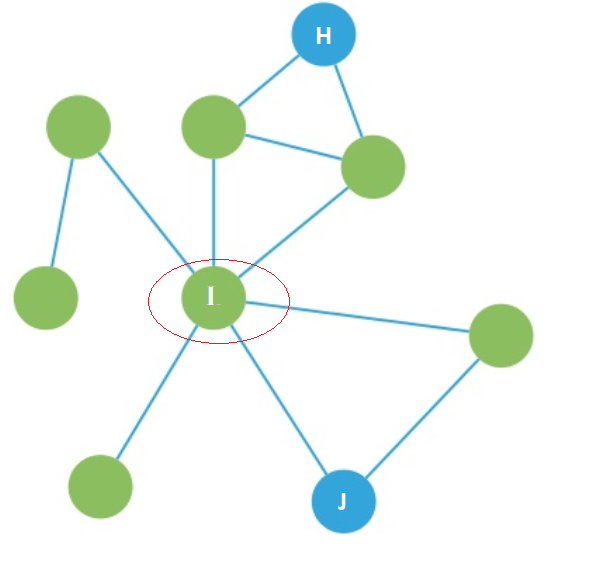
\includegraphics[width=8cm]{figs/BC.png}
\label{BC}
\caption{Grafo que representa o conceito de centralidade de intermediação.}
\end{figure}

A centralidade de intermediação é computada de forma equivalente em redes ponderadas e direcionadas, desde que os comprimentos dos caminhos sejam calculados nos respectivos caminhos ponderados ou direcionados.
% ----------------------------------------------------------
% PARTE
% ----------------------------------------------------------
\chapter{Aquisição de dados}
% ----------------------------------------------------------

A epilepsia de ausência na infância é uma epilepsia generalizada não convulsiva idiopática com uma etiologia genética multifatorial \cite{crunelli2002childhood}. Tal patologia é caracterizada principalmente por breves períodos (10s a 30s) de perda de atenção, no qual a criança permanece com olhar fixo e distante e não responde à estímulos externos.

A base de dados foi desenvolvida em parceria com o Hospital Israelita Albert Einstein. Os dados do EEG foram registrados usando o amplificador Ceegraph EEG (Bio-logic Systems Corp, EUA) com taxa de amostragem de 256 Hz e 20 canais no sistema padrão 10/20. As posições dos canais foram: FP1, FP2, F7, F3, Fz, F4 e F8 (córtex frontal); T7, C3, Cz, C4 e T8 (córtex central); P7, P3, Pz, P4, P8, O1, Oz e O2 (córtex posterior). Sua impedância foi mantida abaixo de 10 k $ \Omega $. 

Os dados brutos foram revisados e o período crítico foi marcado por um neurofisiologista clínico certificado pelo conselho. Hiperventilação e estimulação fótica intermitente foram realizadas rotineiramente. Gravações de vigília e sono foram obtidas de 11 pacientes com crises de ausência. 

Deles, selecionamos 17 períodos de apreensão, cada um abrangendo 10 segundos do período inter-ictal (definido por uma atividade de EEG sem anormalidades entre as convulsões) e 10 segundos durante a atividade ictal. Consideramos cada período de apreensão como um episódio independente como em \cite {sadleir2006electroclinical, mormann2003epileptic}.

O pré-processamento foi realizado com o pacote EEGlab (Swartz Center for Computational Neuroscience, EUA) para o Matlab R2013b (Mathworks Inc., EUA). O sinal foi filtrado com um passa banda butterworth de 1 a 31 Hz. Os canais foram referenciados à média comum de todos os eletrodos. Na Fig.~\ref{fig: eeg}  mostramos um exemplo de dados de EEG para os períodos de tempo interictal e ictal.

A aprovação do comitê de ética não foi necessária porque a análise foi baseada em dados de epilepsia de ausência retrospectivos anônimos.


\begin{figure}[h]
\centering
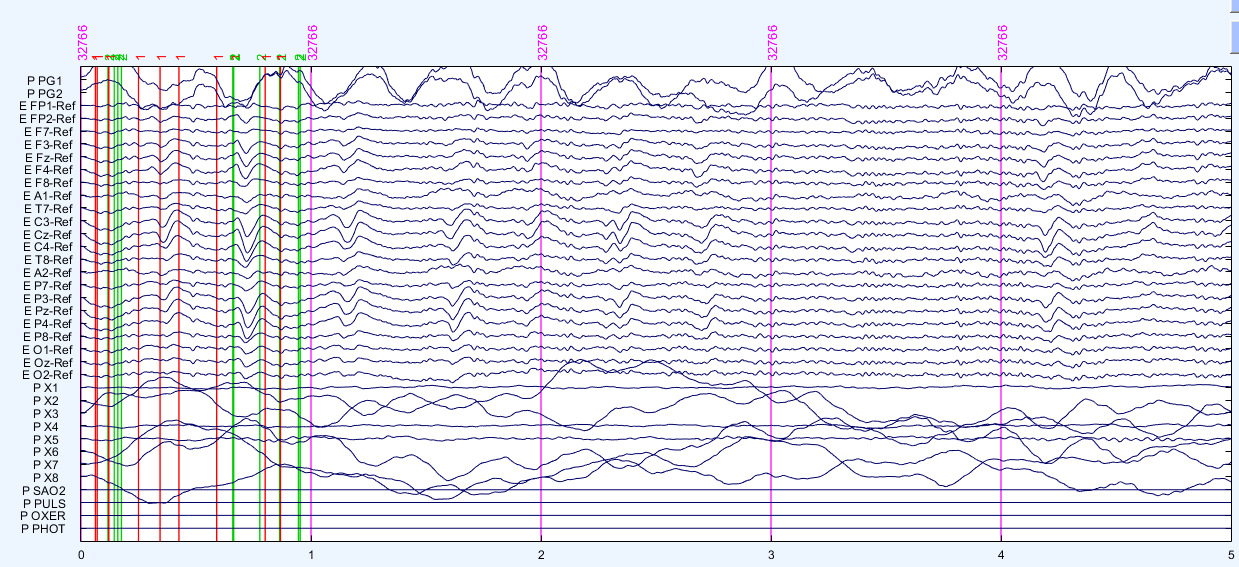
\includegraphics[width=17cm]{figs/EEG-Joao-1.PNG}
\label{fig: eeg}
\caption{Exemplo de EEG de um paciente com crise de ausência em que o tempo inicial e final da crise foi demarcado (linhas vermelha e verde, respectivamente) por um neurologista.}
\end{figure}



\begin{figure}[h]
\centering
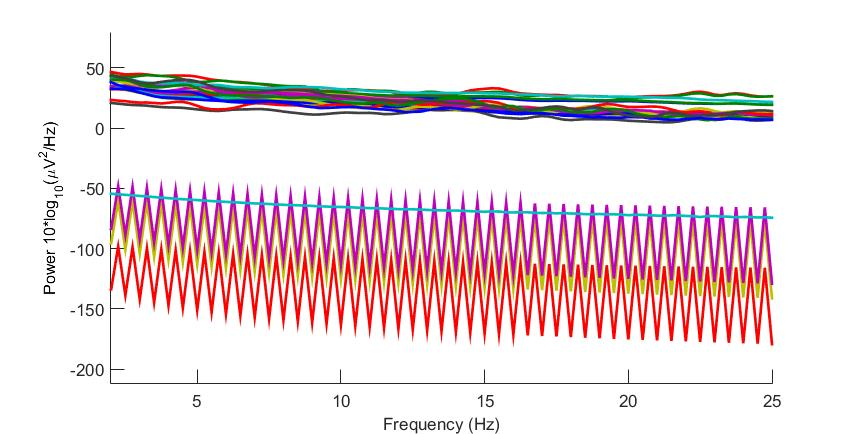
\includegraphics[width=17cm]{figs/Spectro_Joao_1.jpg}
\caption{Análise Espectral do sinal de EEG apresentado acima.}
\label{espectro}
\end{figure}


As crises foram então separadas em 3 momentos: pré-ictal, ictal e pós-ictal. Cada janela possui 12s de duração com 80\% de sobreposição entre elas. Ou seja, cada janela de 12s tem 9,6s exatamente iguais a janela posterior. Esse overlapping foi feito para suavizar os resultados.

Por fim, a base de dados foi criada com dados de 11 pacientes, com os 20 canais  dividos em 3 subconjuntos: Pre-Ictal, Ictal e Pos-Ictal. Dada a frequencia de amostragem 256 Hz, cada subconjunto corresponde a uma matriz de dados de 20 x 3072 amostras.

Os eletrodos foram posicionados utilizando o sistema 10-20 de posicionamento, conforme figura abaixo. 

\begin{figure}[h]
\centering
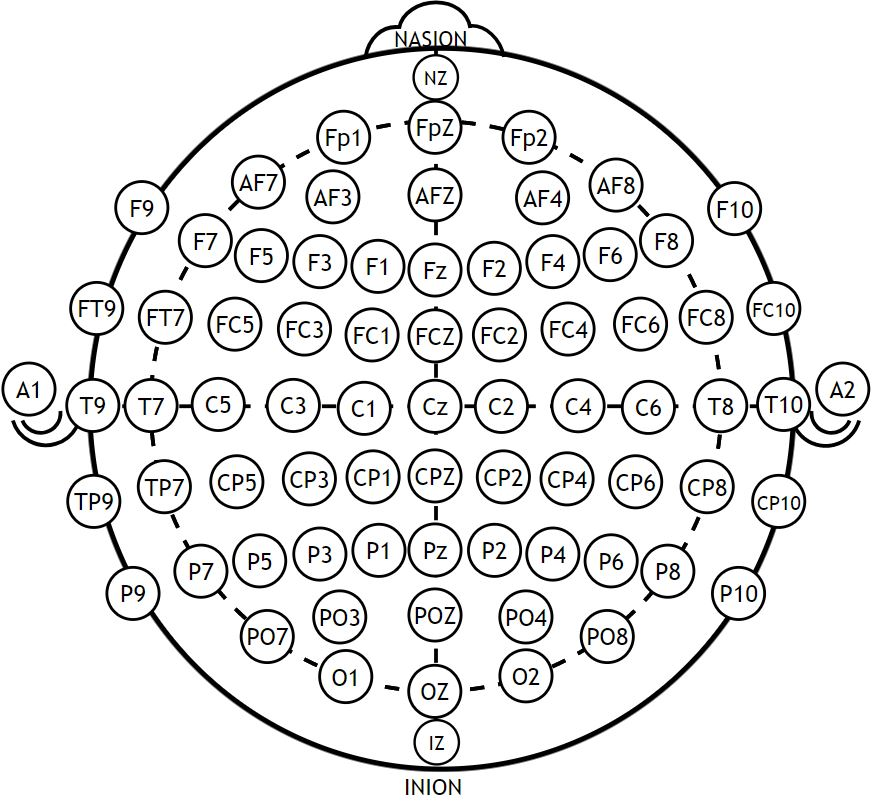
\includegraphics[width=8cm]{figs/10-20.JPG}
\caption{Padrão internacional do sistema 10-20 para EEG.}
\label{fig: 10-20}
\end{figure}

Os eletrodos são nomeados de acordo com a sua posição anatômica. Desta forma, a letra maiúscula que inicia a sigla do eletrodo representa o lóbulo do cérebro sobre o qual ele está posicionado. A figura ~\ref{fig: lobulos} ilustra todos os lóbulos bem como a respectiva nomenclatura e inicial a ser utilizada no eletrodo. 

\begin{figure}[h]
\centering
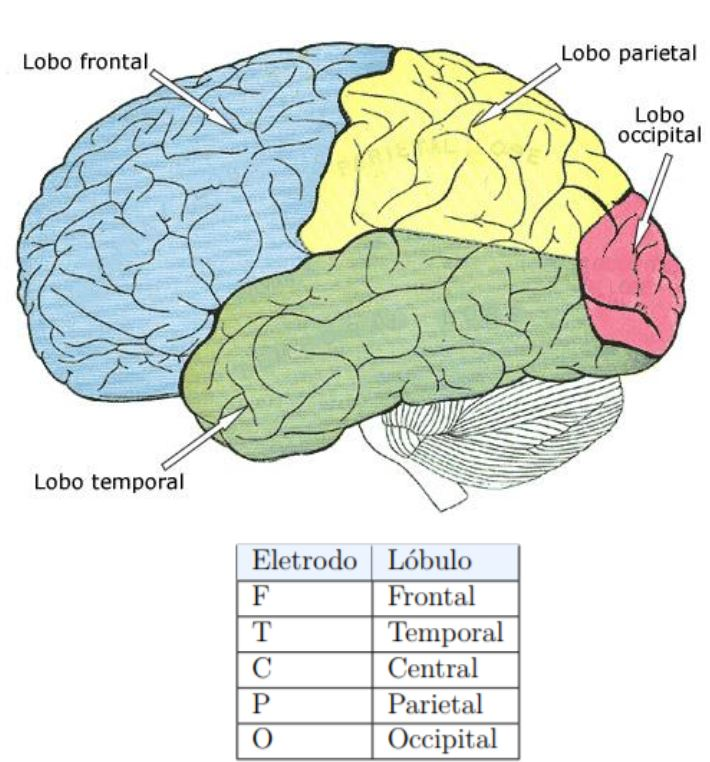
\includegraphics[width=8cm]{figs/lobulos.JPG}
\caption{Lóbulos cerebrais e nomeclatura de eletrodos.}
\label{fig: lobulos}
\end{figure}

Para fins numéricos, cada eletrodo foi associado a um índice numérico de canal. A tabela ~\ref{table: eletrodos} explicita a relação entre canal e eletrodo. De forma que o índice do canal 1 corresponde ao eletrodo "Fp1", o índice do canal 2 corresponde ao eletrodo "Fp2" e assim sucessivamente. As letras maiúsculas iniciais dizem respeito a localização anatômica do eletrodo. 

Desta forma, para todos os gráficos contidos neste trabalho, onde o eixo do canal possuir valor 1, significa que aquele canal corresponde ao eletrodo "Fp1" que encontra-se localizado no lóbulo frontal.

\begin{table}[h]
\caption{Relação entre índices numéricos dos canais e eletrodos}
\centering
\begin{tabular}{cclll}

Eletrodo                  & Canal                   &                      &                      &  \\ \cline{1-2}
\multicolumn{1}{|c|}{Fp1} & \multicolumn{1}{c|}{1}  & \multicolumn{1}{c}{} & \multicolumn{1}{c}{} &  \\ \cline{1-2}
\multicolumn{1}{|c|}{Fp2} & \multicolumn{1}{c|}{2}  & \multicolumn{1}{c}{} & \multicolumn{1}{c}{} &  \\ \cline{1-2}
\multicolumn{1}{|c|}{F7}  & \multicolumn{1}{c|}{3}  & \multicolumn{1}{c}{} & \multicolumn{1}{c}{} &  \\ \cline{1-2}
\multicolumn{1}{|c|}{F3}  & \multicolumn{1}{c|}{4}  & \multicolumn{1}{c}{} & \multicolumn{1}{c}{} &  \\ \cline{1-2}
\multicolumn{1}{|c|}{Fz}  & \multicolumn{1}{c|}{5}  &                      &                      &  \\ \cline{1-2}
\multicolumn{1}{|c|}{F4}  & \multicolumn{1}{c|}{6}  &                      &                      &  \\ \cline{1-2}
\multicolumn{1}{|c|}{F8}  & \multicolumn{1}{c|}{7}  &                      &                      &  \\ \cline{1-2}
\multicolumn{1}{|c|}{T7}  & \multicolumn{1}{c|}{8}  &                      &                      &  \\ \cline{1-2}
\multicolumn{1}{|c|}{C3}  & \multicolumn{1}{c|}{9}  &                      &                      &  \\ \cline{1-2}
\multicolumn{1}{|c|}{Cz}  & \multicolumn{1}{c|}{10} &                      &                      &  \\ \cline{1-2}
\multicolumn{1}{|c|}{C4}  & \multicolumn{1}{c|}{11} &                      &                      &  \\ \cline{1-2}
\multicolumn{1}{|c|}{T8}  & \multicolumn{1}{c|}{12} &                      &                      &  \\ \cline{1-2}
\multicolumn{1}{|c|}{P7}  & \multicolumn{1}{c|}{13} &                      &                      &  \\ \cline{1-2}
\multicolumn{1}{|c|}{P3}  & \multicolumn{1}{c|}{14} &                      &                      &  \\ \cline{1-2}
\multicolumn{1}{|c|}{Pz}  & \multicolumn{1}{c|}{15} &                      &                      &  \\ \cline{1-2}
\multicolumn{1}{|c|}{P4}  & \multicolumn{1}{c|}{16} &                      &                      &  \\ \cline{1-2}
\multicolumn{1}{|c|}{P8}  & \multicolumn{1}{c|}{17} &                      &                      &  \\ \cline{1-2}
\multicolumn{1}{|c|}{O1}  & \multicolumn{1}{c|}{18} &                      &                      &  \\ \cline{1-2}
\multicolumn{1}{|c|}{Oz}  & \multicolumn{1}{c|}{19} &                      &                      &  \\ \cline{1-2}
\multicolumn{1}{|c|}{O2}  & \multicolumn{1}{c|}{20} &                      &                      &  \\ \cline{1-2}
\label{table: eletrodos}
\end{tabular}
\end{table}





% ----------------------------------------------------------
% PARTE
% ----------------------------------------------------------
\chapter{Resultados}
% ----------------------------------------------------------
O procedimento adotado para análise dos dados foi:
\begin{itemize}
    \item Cálculo das matrizes de adjacência
    \item Cálculo dos parâmetros de Rede
    \item Idêntificação dos Hubs
    \item Análises estatísticas dos Hubs
    \item Análises anatômicas dos Hubs
\end{itemize}
Cada item será descrito e explicitado nas seções a seguir. Para cada tipo de análise, os dados utilizados foram os mesmos, apenas a metodologia variou. No caso do PLV, apesar de haver propostas de que análises com lag $\neq 0$, todas as análises foram feitas com lag = 0 para manter a característica não-direcional da medida.

\section{Cálculo da Matriz de Adjacência}

As matrizes de adjacência foram calculadas a partir de scripts MatLab que implementam numericamente as equações definidas na seção 1. Foram utilizados 20 dos 32 canais disponíveis e, para efeitos de cálculo, os eletrodos foram mapeados conforme a Tabela ~\ref{table: eletrodos}.

As Figuras ~\ref{PLV_11pcts} e ~\ref{TE_11pctes} representam os resultados obtidos para cada caso. Percebe-se, para o caso da Entropia de Transferência, na Figura ~\ref{TE_11pctes}, que o paciente 1 apresentou valores muito divergentes (alguns até negativos) em relação aos demais.
A primeira intenção foi de normalizar todos os resultados, tal qual feito para o PLV. Percebeu-se, porém, que na verdade tratava-se de um resultado espúrio e poderia então ser relevado para fins de análises.
Nos demais pacientes, a direcionalidade da informação fica bastante evidente.

Já no caso do PLV, não é possível perceber direcionalidade da informação (gráfico simétrico). Além disso, não é possível isolar visualmente uma determinada área de maior conexão.

Essa mesma análise visual também é custosa no caso da entropia de transferência. Desta forma, o próximo passo foi a determinação dos hubs por meio da centralidade de proximidade.

\begin{sidewaysfigure}

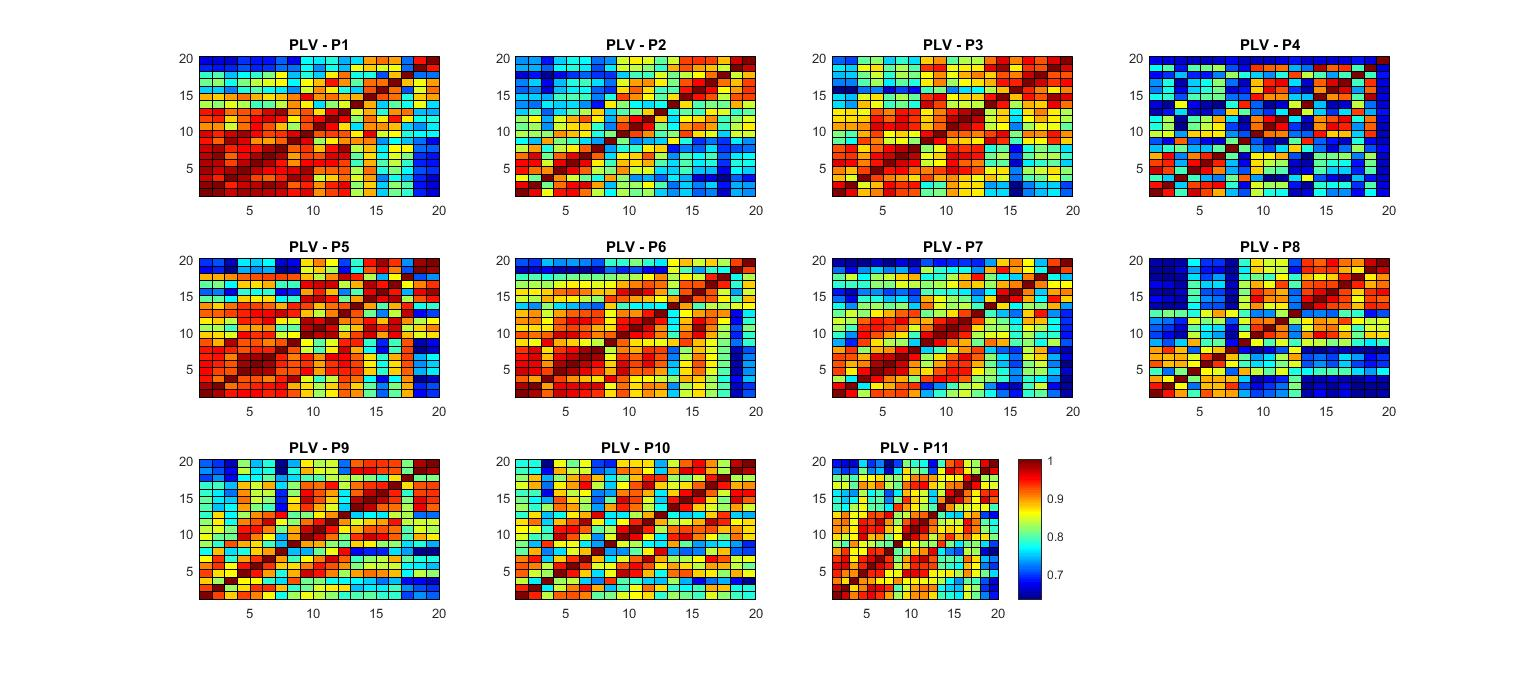
\includegraphics[width=26cm]{figs/plv_todospcts.jpg}
\label{PLV_11pcts}
\caption{PLV a lag 0 para os 11 pacientes.Cada eixo contém os 20 canais e os resultados estão normalizados em que 1 representa a maior sincronização entre dois canais.}
\end{sidewaysfigure}

\begin{sidewaysfigure}
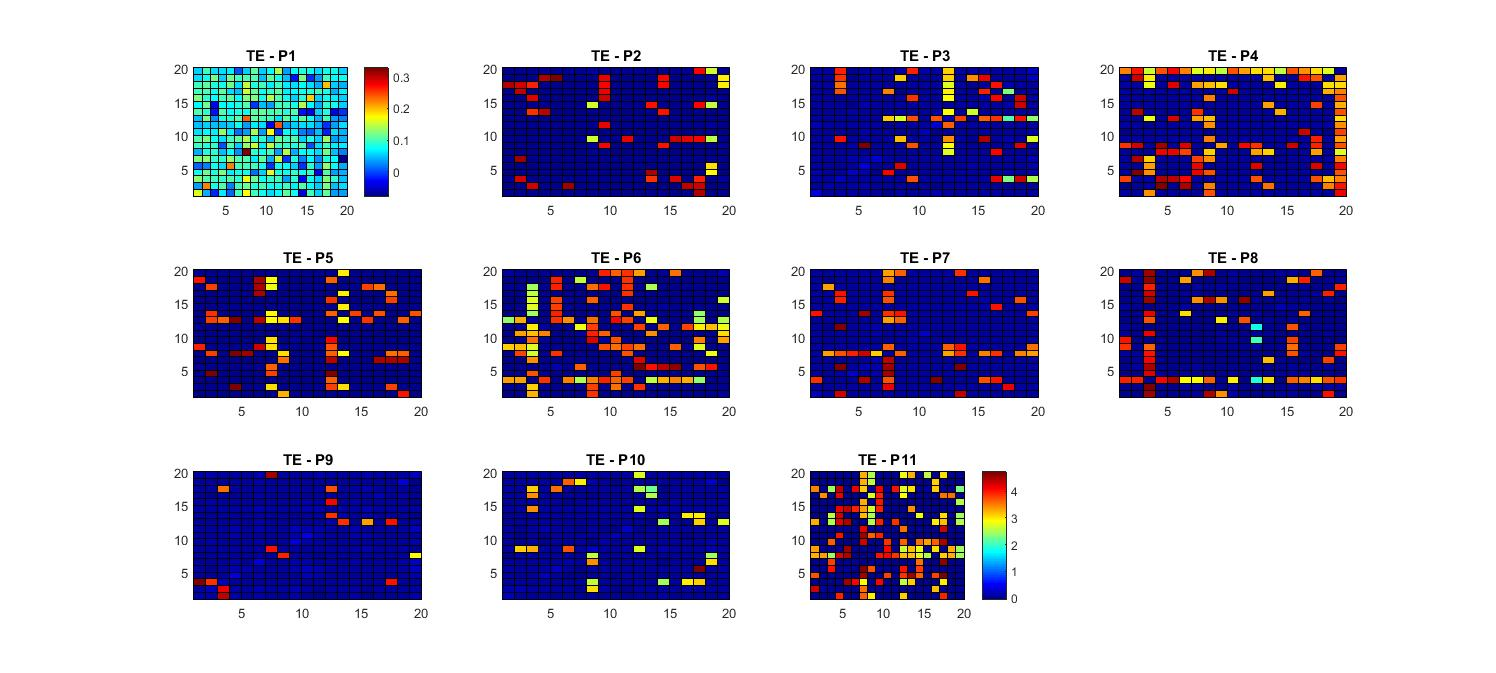
\includegraphics[width=25cm]{figs/Figure_TE_11pctes.jpg}
\label{TE_11pctes}
\caption{Entropia de transferência para os 11 pacientes. Cada eixo contém os 20 canais e o tom de vermelho mais escuro para os pacientes de 2 a 11 corresponde a 5.}
\end{sidewaysfigure}

\section{Cálculo dos parâmetros de rede}

A partir do cálculo realizado com o toolkit para MatLab disponibilizado por Sporns \cite{rubinov2010complex}, foi possível determinar os hubs para cada paciente durante o período ictal. As figuras a seguir apresentam os resultados obtidos.

Percebe-se que o PLV evidencia mais a região central e a Entropia de Transferência as regiões frontal e parietal. Além disso, é possível perceber também que a quantidade de hubs por paciente em geral é a mesma para ambos os casos.

Por outro lado, a entropia de transferência é bem mais precisa no sentido de que: sabe-se que a região central do cérebro é responsável por um grande fluxo de informação por conectar funcionalmente partes anatomicamente "desconectadas" e o PLV confirma isso. A entropia de trasnferência identifica os hubs em suas áreas mais espcificas.

\begin{figure}[h]
\centering
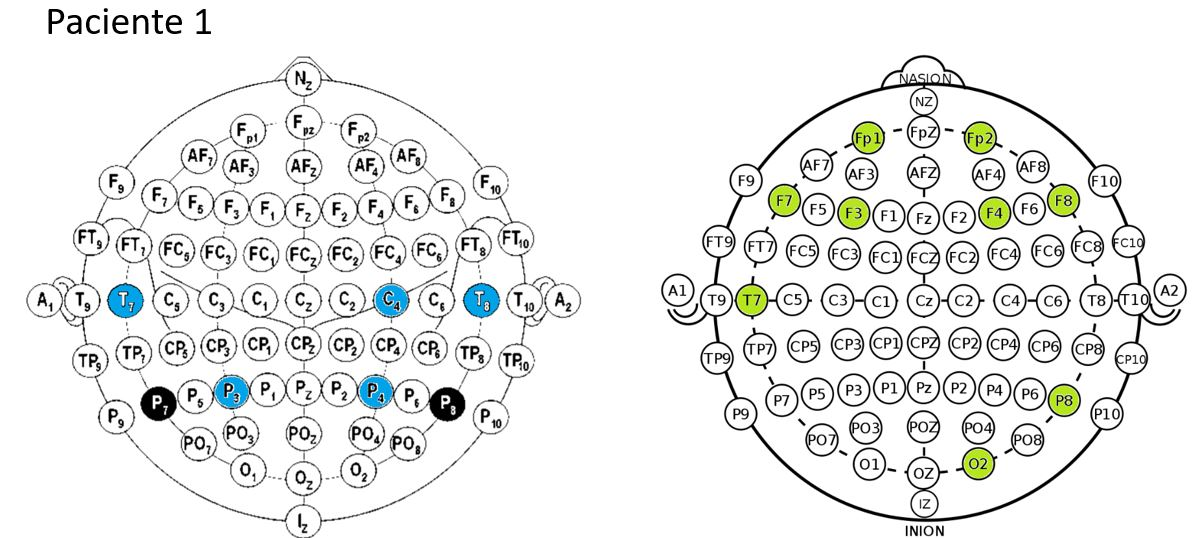
\includegraphics[width=17cm]{figs/p1.JPG}
\label{eeg}
\caption{PLV (em azul) e Entropia de Transferência (em verde) para o paciente 1.}
\end{figure}

\begin{figure}[]
\centering
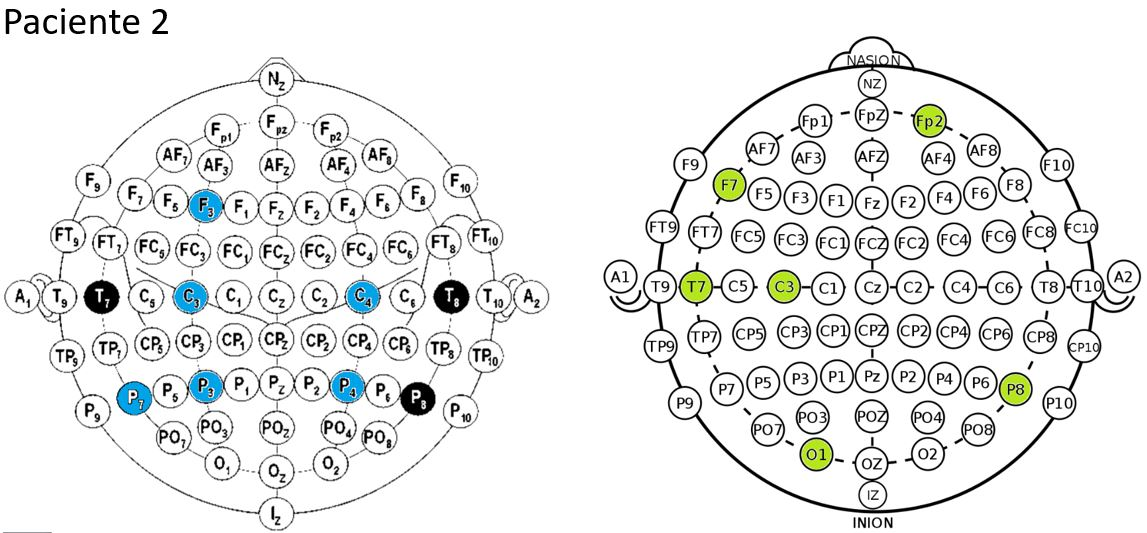
\includegraphics[width=17cm]{figs/p2.JPG}
\label{eeg}
\caption{PLV (em azul) e Entropia de Transferência (em verde) para o paciente 2.}
\end{figure}

\begin{figure}[]
\centering
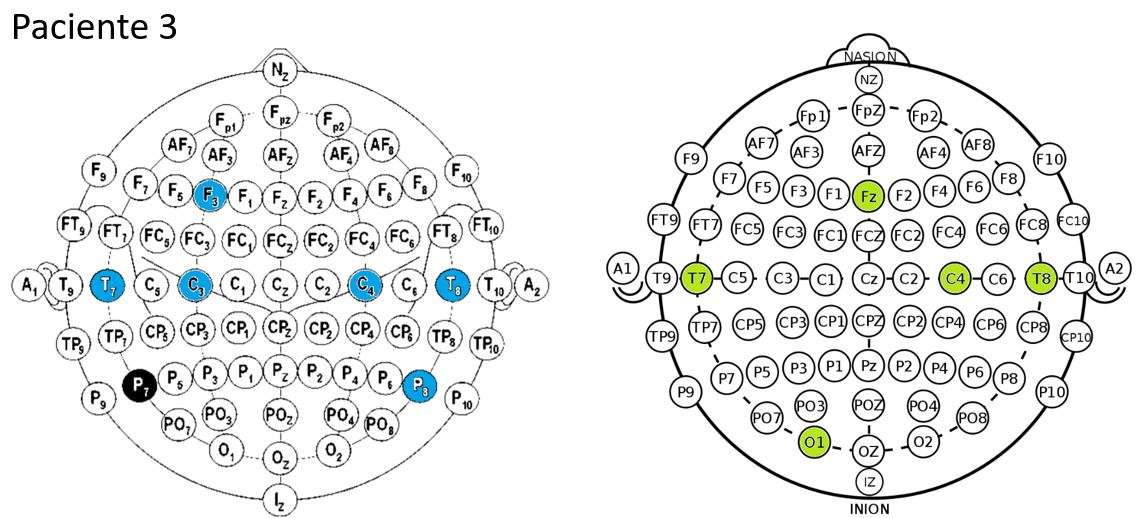
\includegraphics[width=17cm]{figs/p3.JPG}
\label{eeg}
\caption{PLV (em azul) e Entropia de Transferência (em verde) para o paciente 3.}
\end{figure}

\begin{figure}[]
\centering
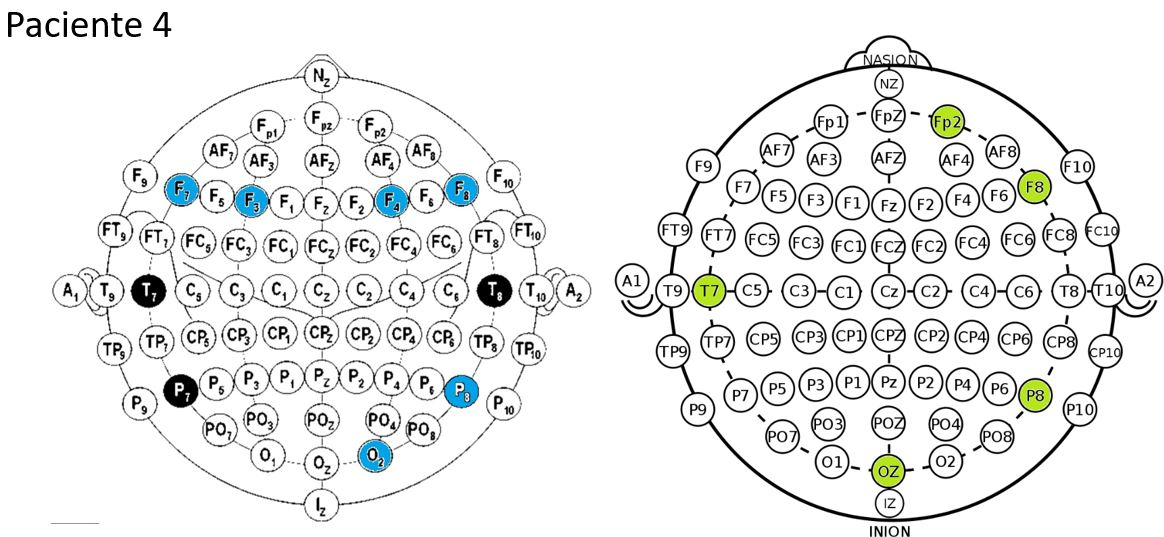
\includegraphics[width=17cm]{figs/p4.JPG}
\label{eeg}
\caption{PLV (em azul) e Entropia de Transferência (em verde) para o paciente 4.}
\end{figure}

\begin{figure}[]
\centering
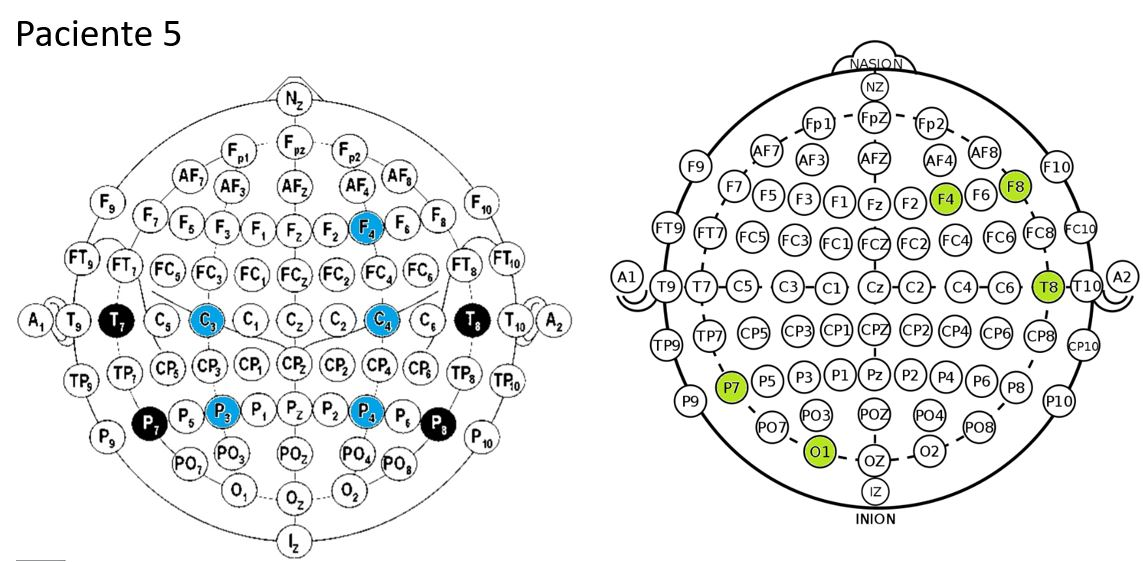
\includegraphics[width=17cm]{figs/p5.JPG}
\label{eeg}
\caption{PLV (em azul) e Entropia de Transferência (em verde) para o paciente 5.}
\end{figure}

\begin{figure}[]
\centering
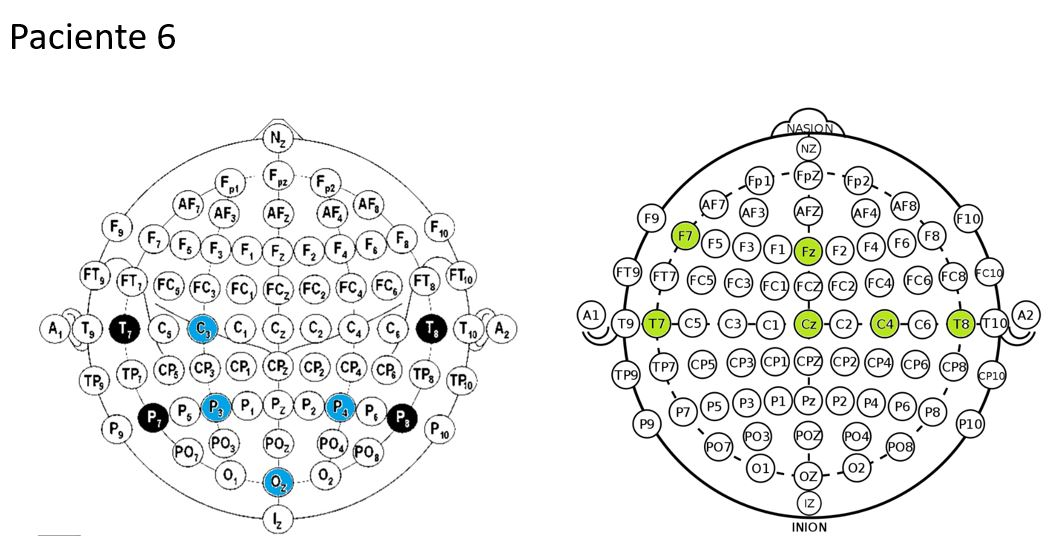
\includegraphics[width=17cm]{figs/p6.JPG}
\label{eeg}
\caption{PLV (em azul) e Entropia de Transferência (em verde) para o paciente 6.}
\end{figure}

\begin{figure}[]
\centering
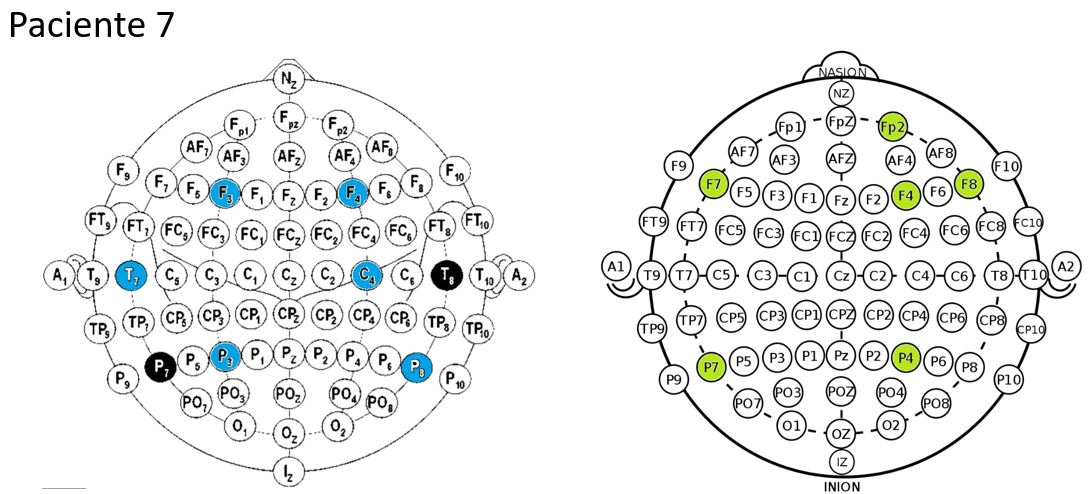
\includegraphics[width=17cm]{figs/p7.JPG}
\label{eeg}
\caption{PLV (em azul) e Entropia de Transferência (em verde) para o paciente 7.}
\end{figure}

\begin{figure}[]
\centering
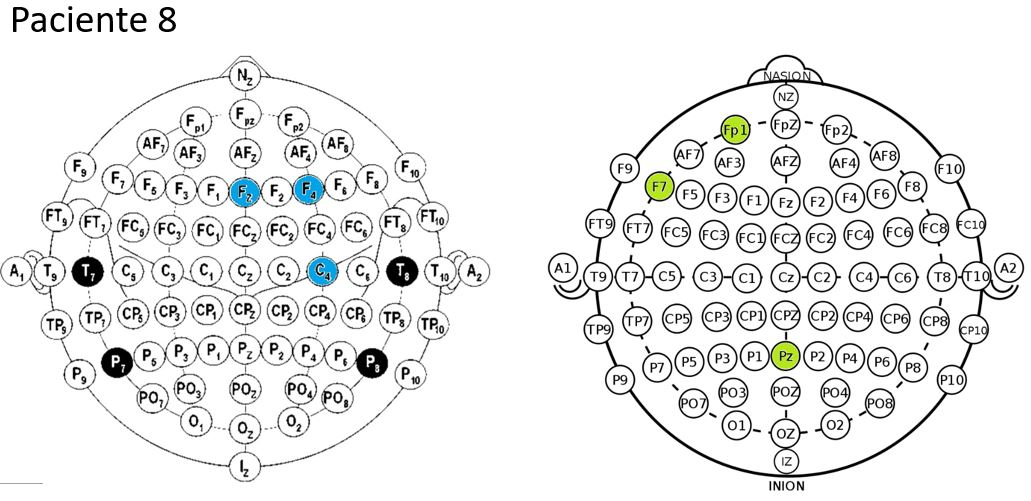
\includegraphics[width=17cm]{figs/p8.JPG}
\label{eeg}
\caption{PLV (em azul) e Entropia de Transferência (em verde) para o paciente 8.}
\end{figure}

\begin{figure}[]
\centering
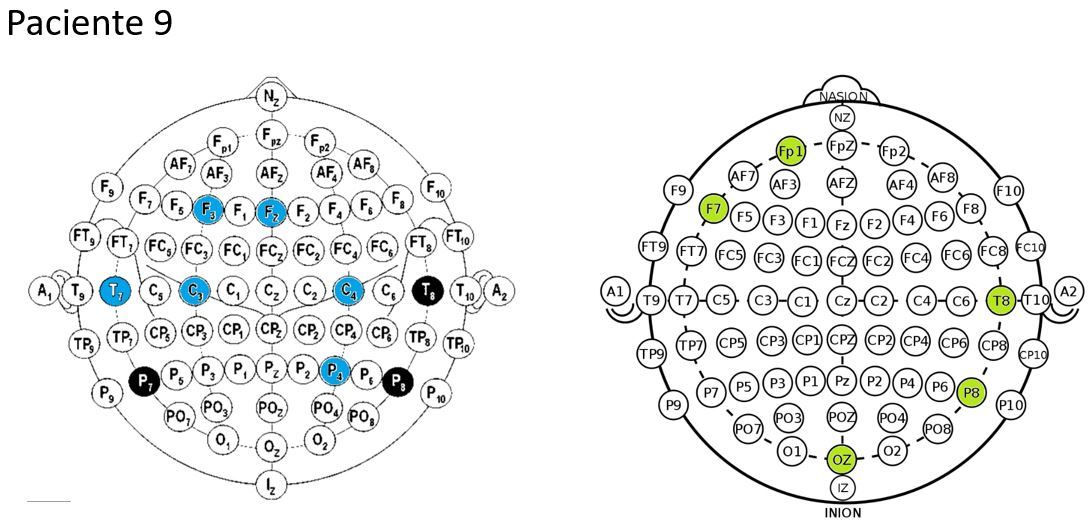
\includegraphics[width=17cm]{figs/p9.JPG}
\label{eeg}
\caption{PLV (em azul) e Entropia de Transferência (em verde) para o paciente 9.}
\end{figure}

\begin{figure}[]
\centering
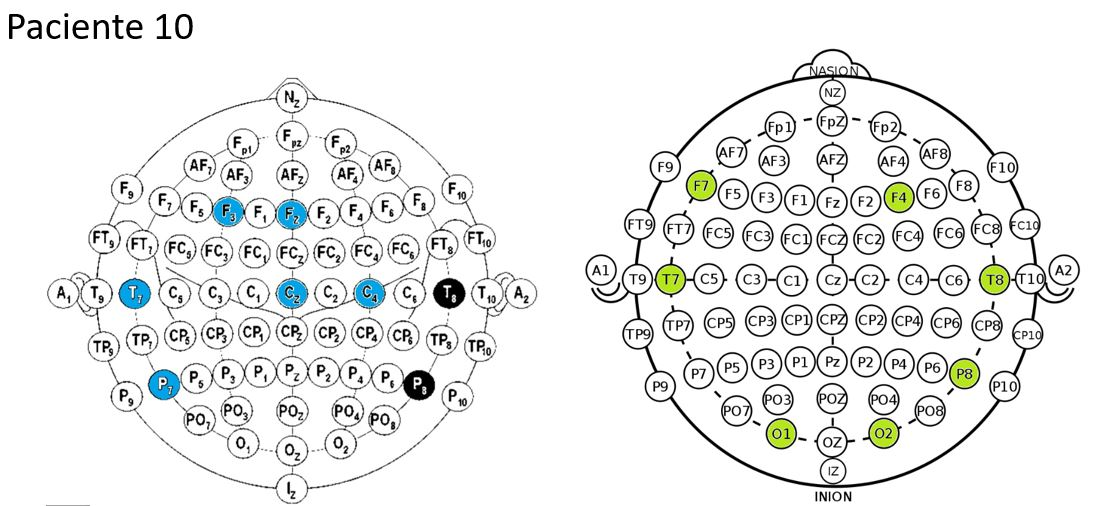
\includegraphics[width=17cm]{figs/p10.JPG}
\label{eeg}
\caption{PLV (em azul) e Entropia de Transferência (em verde) para o paciente 10.}
\end{figure}

\begin{figure}[]
\centering
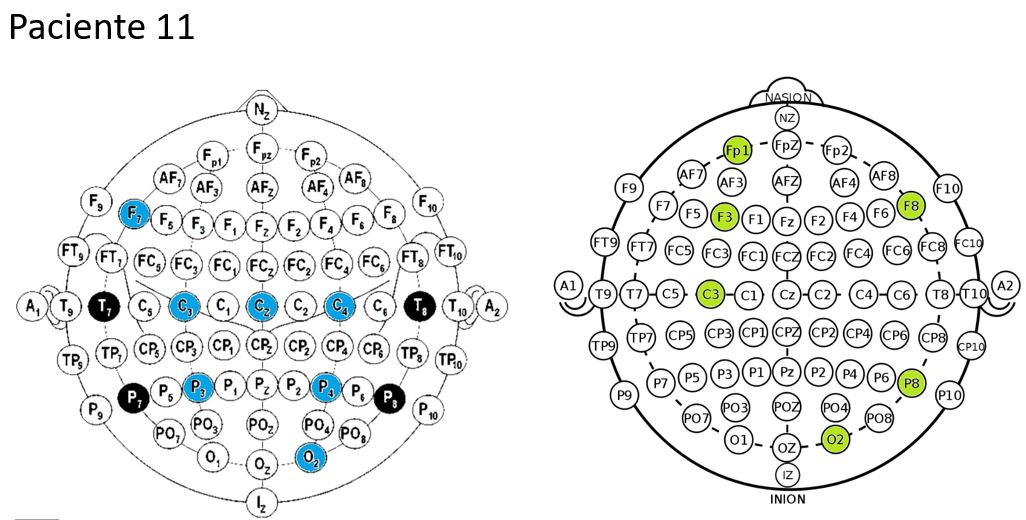
\includegraphics[width=17cm]{figs/p11.JPG}
\label{eeg}
\caption{PLV (em azul) e Entropia de Transferência (em verde) para o paciente 11.}
\end{figure}

\section{Análises estatísticas dos Hubs}

Após a identificação dos hubs, uma análise estatística foi realizada e os resultados podem ser observados nas figuras a seguir.

\begin{figure}[h]
\centering
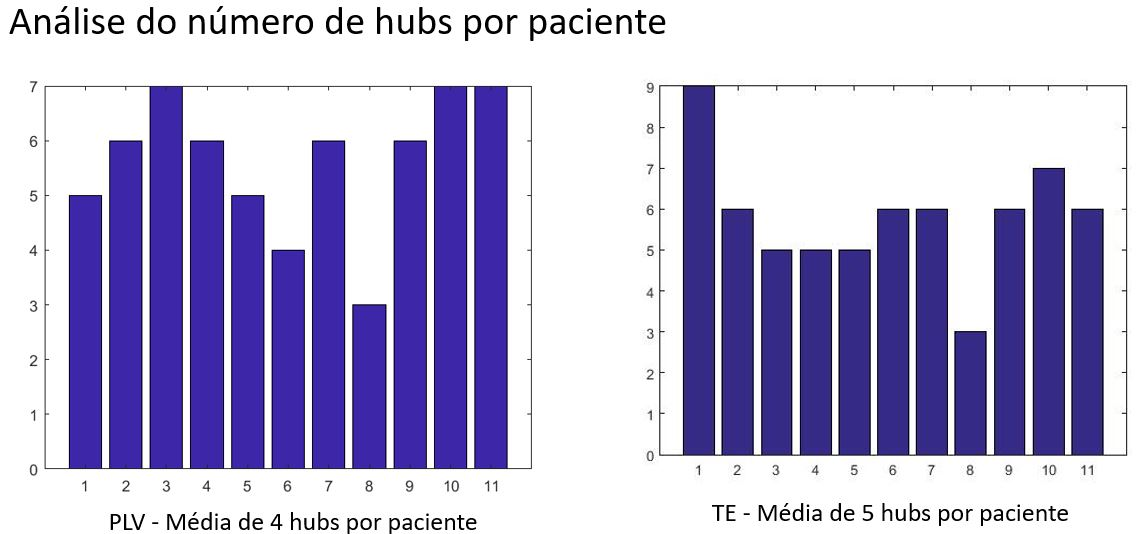
\includegraphics[width=15cm]{figs/hubsporpcte.JPG}
\label{eeg}
\caption{Número de "hubs" identificados por paciente.}
\end{figure}

Além disso, analisou-se a frequência com que um dado canal era identificado como hub. Os resultados estão na figura a seguir.
\begin{figure}[h]
\centering
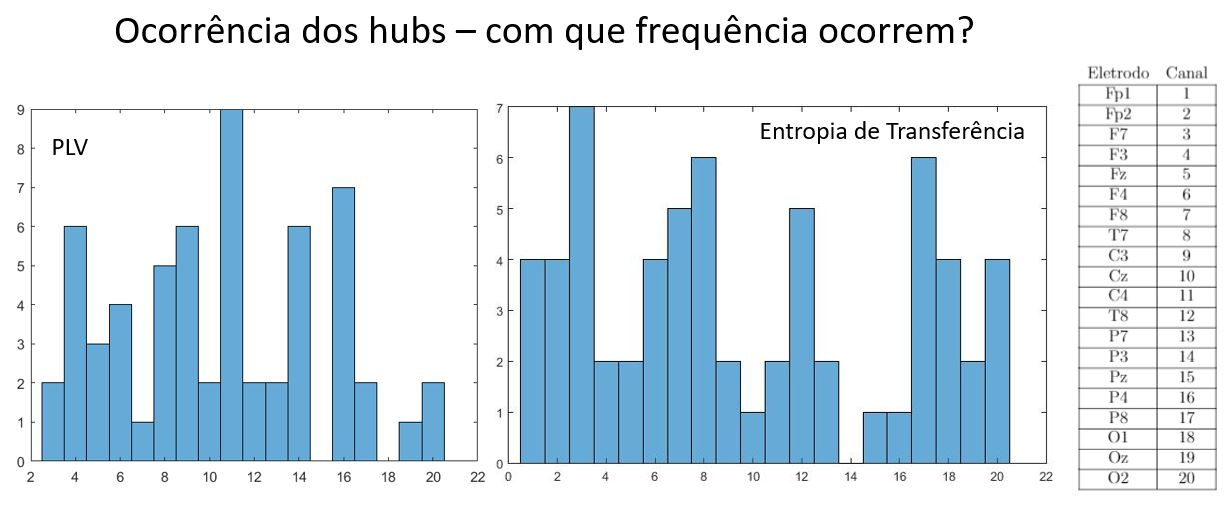
\includegraphics[width=15cm]{figs/freq.JPG}
\label{eeg}
\caption{Frequência com que um eletrodo é identificado como "hub".}
\end{figure}

Percebe-se que ambas métricas identificaram aproximadamente o mesmo número de hubs, porém a entropia de transferência definiu melhor a região dos hubs. Enquanto o PLV identifica basicamente as estruturas centrais, a entropia de transferência identifica regiões específicas e bem definidas nas regiões frontal e parietal.



% ---


% ----------------------------------------------------------
% Finaliza a parte no bookmark do PDF
% para que se inicie o bookmark na raiz
% e adiciona espaço de parte no Sumário
% ----------------------------------------------------------
%\phantompart

% ---
% Conclusão (outro exemplo de capítulo sem numeração e presente no sumário)
% ---
\chapter*[Conclusão]{Conclusão}
\addcontentsline{toc}{chapter}{Conclusão}
% ---

As análises mostram que crises generalizadas de epilepsia (crises de ausência), apesar do alto nível de sincronismo, possuem regiões de maior conectividade bem definidas. Medidas de informação direcionais e não-direcionais podem ser utilizadas para identificar tais regiões.

Apesar de apresentarem regiões anatômicas diferentes, tanto o PLV quanto a entropia de transferência identificaram aproximadamente o mesmo número de hubs: 5 por paciente.

As análises do PLV foram feitas apenas para as séries sem atraso (lag = 0). Talvez com informações de sincronização (lag $\neq 0$), seja possível se aproximar mais dos resultados obtidos com a entropia de transferência.

Como a natureza do código neuronal permanece desconhecida, as propriedades de cada método levam a topologias de rede distintas. Porém todas elas podem ser úteis para melhor caracterizar as diferentes patologias neuronais de maneira complementar.

Há de se levar em conta que os dados apresentados neste trabalho dão indícios do comportamento dos métodos utilizados porém como o espaço amostral foi consideravelmente pequeno, não é possível inferir com precisão sobre a região anatômica de maior conectividade na crise de ausência. Seria necessário muito mais dados de pacientes para que as infereências fossem estatitisticamente relevantes.

Por fim, os objetivos do trabalho foram atingidos e os resultados obtidos devidamente discutidos.



% ----------------------------------------------------------
% ELEMENTOS PÓS-TEXTUAIS
% ----------------------------------------------------------
%\postextual
% ----------------------------------------------------------

% ----------------------------------------------------------
% Referências bibliográficas
% ----------------------------------------------------------
\bibliography{bib-ref}

\end{document}
